\documentclass{beamer}
\usetheme{Madrid}

\title{About Machine Learning}
\author{by Amit Swain}
\centering
\date{September 2019}
\begin{document}
\maketitle
\begin{frame}{Content}
\begin{itemize}
\item What is machine learning? 
\item Growth of Machine Learning.
\item Application of machine Learning. 
\item Classification:  Applications
 \item Top 10 use cases of Machine Learning
 \item What machine learning tools do Kaggle champions use?
    \item Types of Learning? 
\end{itemize}
\end{frame}
\begin{frame}{What is Machine learning?}
\framesubtitle{Why do we need to care about machine learning?}
\begin{itemize}
    \item Machine learning (ML) is a category of algorithm that allows software applications to become more accurate in predicting outcomes without being explicitly programmed. The basic premise of machine learning is to build algorithms that can receive input data and use statistical analysis to predict an output while updating outputs as new data becomes available.
    \item Writing software is the bottleneck, we don’t have enough good developers. Let the data do the work instead of people. Machine learning is the way to make programming scalable.
    \item Machine Learning is getting computers to program themselves. If programming is automation, then machine learning is automating the process of automation.
\end{itemize}
\end{frame}
\begin{frame}{Growth of Machine Learning}
   \begin{itemize}
       \item Machine learning is preferred approach to
       \item Speech recognition, Natural language processing
       \item Computer vision
       \item Medical outcomes analysis
    \item Robot control
    \item Computational biology
    \item Improved machine learning algorithms
    \item Improved data capture, networking, faster computers
    \item Software too complex to write by hand
    \item New sensors / IO devices
\end{itemize}
\end{frame}

\begin{frame}{Applications of Machine Learning}
  \framesubtitle{Sample applications of machine learning:}
  The value of machine learning technology has been recognized by companies across several industries that deal with huge volumes of data. By leveraging insights obtained from this data, companies are able work in an efficient manner to control costs as well as get an edge over their competitors. This is how some sectors / domains are implementing machine learning -
  \begin{itemize}
      \item Financial Services
      \item Marketing and Sales
      \item Government
      \item Healthcare
      \item Transportation
      \item Oil and Gas
  \end{itemize}
 
\end{frame}
\begin{frame}
\frametitle{Sample application of Machine Learning}
 
\begin{block}{Financial Services}
Companies in the financial sector are able to identify key insights in financial data as well as prevent any occurrences of financial fraud, with the help of machine learning technology. The technology is also used to identify opportunities for investments and trade. Usage of cyber surveillance helps in identifying those individuals or institutions which are prone to financial risk, and take necessary actions in time to prevent fraud.
\end{block}
 
\begin{block}{Marketing and Sales}
Companies are using machine learning technology to analyze the purchase history of their customers and make personalized product recommendations for their next purchase. This ability to capture, analyze, and use customer data to provide a personalized shopping experience is the future of sales and marketing.
\end{block}
\end{frame}
\begin{frame}
\begin{block}{Government}
Government agencies like utilities and public safety have a specific need FOR Ml, as they have multiple data sources, which can be mined for identifying useful patterns and insights. For example sensor data can be analyzed to identify ways to minimize costs and increase efficiency. Furthermore, ML can also be used to minimize identity thefts and detect fraud.
\end{block}
\begin{block}{Healthcare}
With the advent of wearable sensors and devices that use data to access health of a patient in real time, ML is becoming a fast-growing trend in healthcare. Sensors in wearable provide real-time patient information, such as overall health condition, heartbeat, blood pressure and other vital parameters. Doctors and medical experts can use this information to analyze the health condition of an individual, draw a pattern from the patient history, and predict the occurrence of any ailments in the future. The technology also empowers medical experts to analyze data to identify trends that facilitate better diagnoses and treatment.
\end{block}
\end{frame}
\begin{frame}
    \begin{block}{Transportation}
    Based on the travel history and pattern of traveling across various routes, machine learning can help transportation companies predict potential problems that could arise on certain routes, and accordingly advise their customers to opt for a different route. Transportation firms and delivery organizations are increasingly using machine learning technology to carry out data analysis and data modeling to make informed decisions and help their customers make smart decisions when they travel.
    \end{block}
    \begin{block}{Oil and Gas}
    This is perhaps the industry that needs the application of machine learning the most. Right from analyzing underground minerals and finding new energy sources to streaming oil distribution, ML applications for this industry are vast and are still expanding.
    \end{block}
\end{frame}

\begin{frame}{Classification: Applications}
    \begin{itemize}
        \item Aka Pattern recognition
\item Face recognition: Pose, lighting, occlusion (glasses, beard), make-up, hair style 
\item Character recognition: Different handwriting styles.
\item Speech recognition: Temporal dependency. 
\item Use of a dictionary or the syntax of the language. 
\item Sensor fusion: Combine multiple modalities; eg, visual (lip image) and acoustic for speech
\item Medical diagnosis: From symptoms to illnesses
\item Web Advertizing: Predict if a user clicks on an ad on the Internet.
\end{itemize}
\end{frame}

\begin{frame}{Main Application}
    \begin{itemize}
        \item Face Recognition
        \item Prediction: Regression
        \item Regression Applications
    \end{itemize}
\end{frame}

\begin{frame}{Top 10 use cases of Machine Learning}
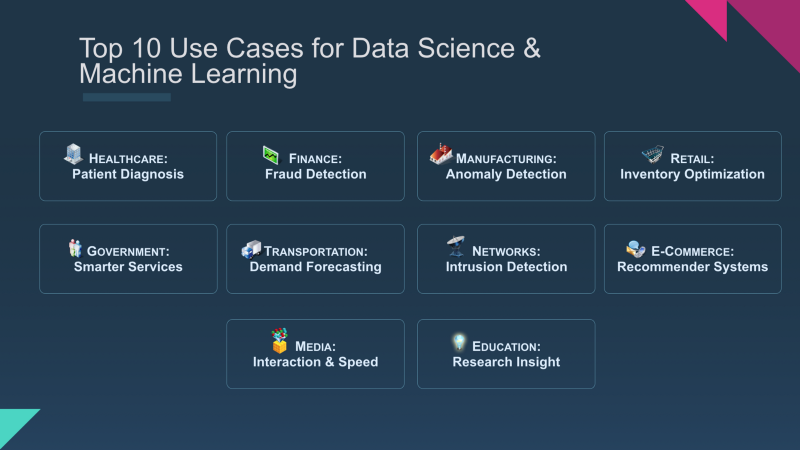
\includegraphics[height=6.8cm]{1_kTnSJQpzGw_w4uQKa_j7VQ.png}
\centering
\end{frame}

\begin{frame}{What machine learning tools do Kaggle champions use?}
 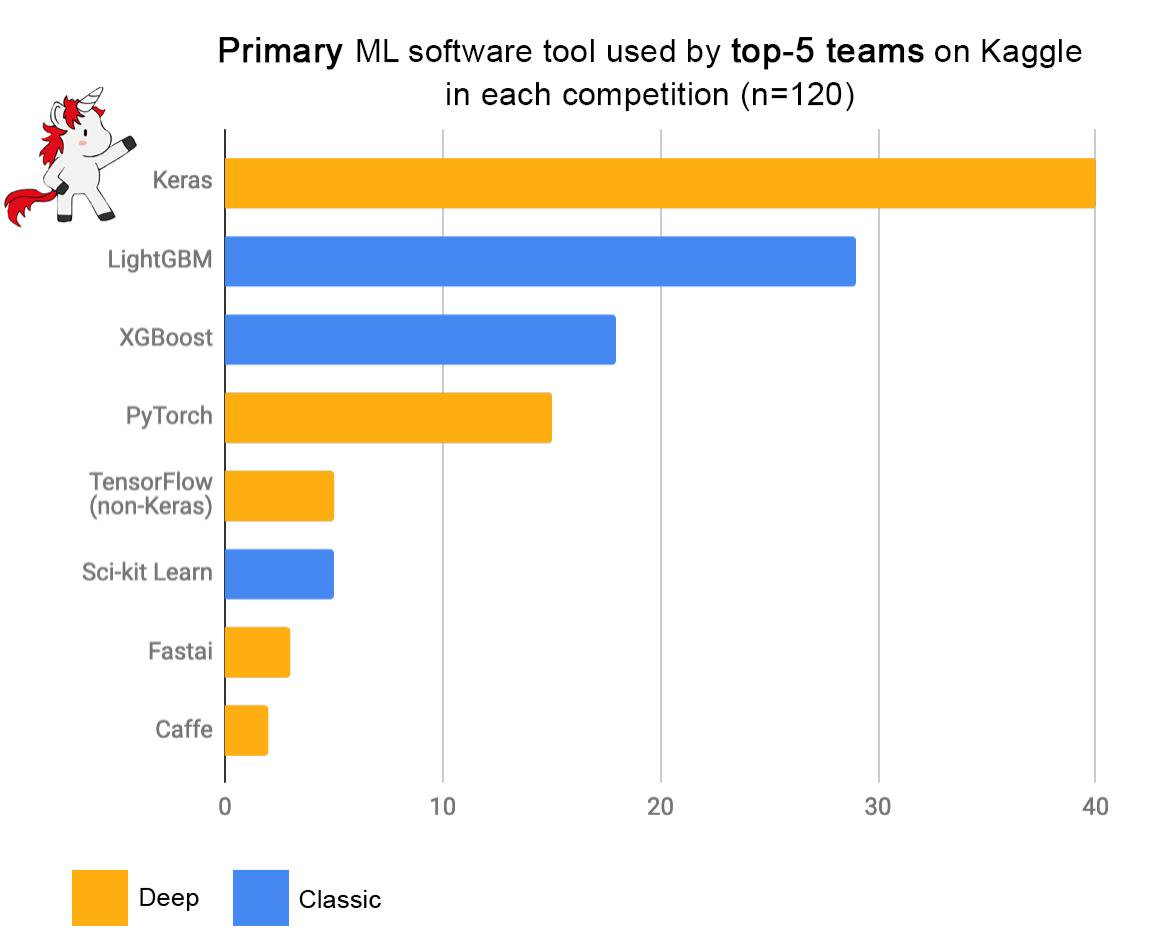
\includegraphics[height=6.8cm]{D3Pb_Q3UIAAuSWU.jpg}
\centering   
\end{frame}

\begin{frame}{Types of Learning?}
\begin{itemize}
    \item Supervised Learning: Uses
    \item Unsupervised Learning
    \item Reinforcement Learning
\end{itemize}
\end{frame}

\begin{frame}{Supervised Learning: Uses}
   \begin{block}{Prediction of future cases}
   Use the rule to predict the output for future inputs
   \end{block}
   \begin{block}{Knowledge extraction}
 The rule is easy to understand
   \end{block}
   \begin{block}{Compression}
  The rule is simpler than the data it explains
   \end{block}
   \begin{block}{Outlier detection}
   Exceptions that are not covered by the rule, e.g., fraud
   \end{block}
  
\end{frame}

\begin{frame}{Unsupervised Learning}
    \begin{itemize}
        \item Learning “what normally happens”
\item No output
\item Clustering: Grouping similar instances
\item Other applications: Summarization, Association Analysis. \end{itemize}
\begin{block}{Example applications}
\begin{itemize}
    \item Customer segmentation in CRM
\item Image compression: Color quantization
\item Bioinformatics: Learning motifs
\end{itemize}
\end{block}
\end{frame}

\begin{frame}{Reinforcement Learning}
    \begin{itemize}
        \item No supervised output but delayed reward
        \item Policies: what actions should an agent take in a particular situation.Utility estimation: how good is a state (used by policy)
        \item Credit assignment problem (what was responsible for the outcome) 
     \end{itemize}
     \begin{block}{Applications}
     \begin{itemize}
        \item Game playing
        \item Robot in a maze
        \item Multiple agents, partial observability, ...
     \end{itemize}
     \end{block}
\end{frame}

\begin{frame}
\huge{\centerline{The End}}
\end{frame}

\end{document}
